\documentclass[11pt]{article}
\usepackage[margin=0.78in]{geometry}
\usepackage{amsmath,amssymb,graphicx,enumitem,multicol,xcolor,fancyhdr}
\usepackage[T1]{fontenc}
\usepackage{url,etoolbox}
% SVG exports already contain PDF transparency groups. Avoid adding a second
% /Group entry with graphics-def 2026; older drivers need no patch.
\makeatletter
\patchcmd{\Gread@pdf}{\Gread@transgrouptrue}{\Gread@transgroupfalse}{}{}
\makeatother
\usepackage[colorlinks=true,urlcolor=blue,linkcolor=black]{hyperref}
\setlength{\headheight}{13.6pt}
\addtolength{\topmargin}{-1.6pt}
\setlength{\parindent}{0pt}
\setlength{\parskip}{5pt}
\setlist[enumerate]{leftmargin=*,itemsep=6pt}
\pagestyle{fancy}
\fancyhf{}
\fancyhead[L]{Mach--Zehnder interferometer}
\fancyhead[R]{Interference and fringe magnification}
\fancyfoot[L]{\scriptsize\thepage}
\fancyfoot[R]{\scriptsize\textcopyright\ 2026 Amy Roberts\quad ORCID: \href{https://orcid.org/0000-0001-8538-9155}{0000-0001-8538-9155}\quad All materials herein \href{https://creativecommons.org/licenses/by/4.0/}{CC BY 4.0}}
\newcommand{\answerline}{\vspace{0.42in}\par\noindent\rule{\linewidth}{0.4pt}}
\newcommand{\answerspace}[1]{\vspace{#1}}
\newcommand{\fig}[2]{\begin{center}\includegraphics[width=#1\linewidth]{figures/#2.pdf}\end{center}}
\begin{document}
\begin{center}
{\LARGE\bfseries From Interference to a Beam Angle}\\[4pt]
{\large A guided investigation of a Mach--Zehnder interferometer}
\end{center}

\textbf{Goal.} Use the spacing between straight, parallel fringes to estimate the small angle between two beams \emph{before} a magnifying lens. Build the result from interference, geometry, and a thin-lens model.

\textbf{Three ways to represent the same linearly polarized plane wave.} The drawings below show three representations of the same electric-field component in space, at a single snapshot in time. The sinusoid plots its value along the direction of propagation; wavefronts mark planes of equal phase; and arrows show the local electric-field direction and magnitude. These are different representations of the same wave, not three different waves.
\begin{center}\vspace{-6pt}
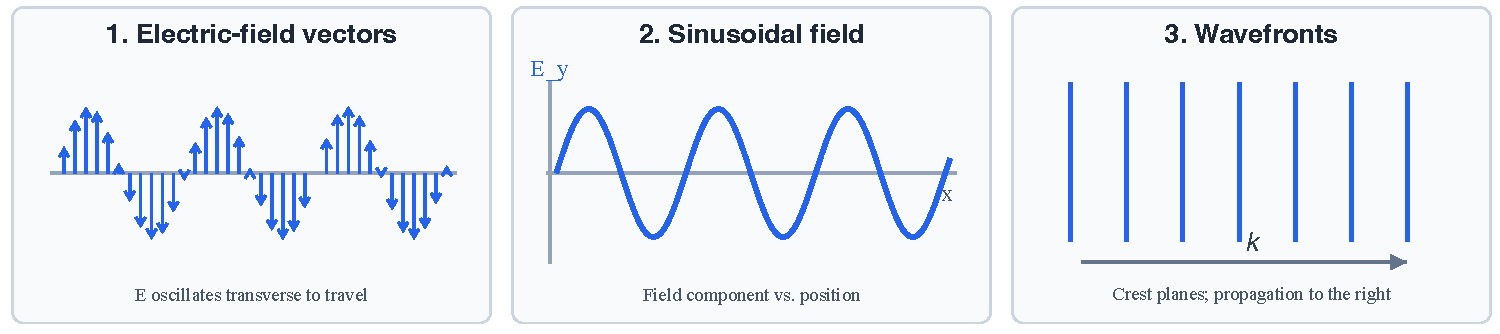
\includegraphics[width=0.98\linewidth]{figures/00_representations.pdf}\vspace{-6pt}\end{center}

\section*{Part A. Constructive and Destructive Interference}
Light is an electromagnetic wave. The sinusoidal curves below represent \emph{one component of the electric field} at a fixed position as time passes (not the physical trajectory of the beam). When two coherent waves with the same polarization overlap, their electric-field components add: $E_{\rm total}=E_1+E_2$.
\begin{center}\vspace{-6pt}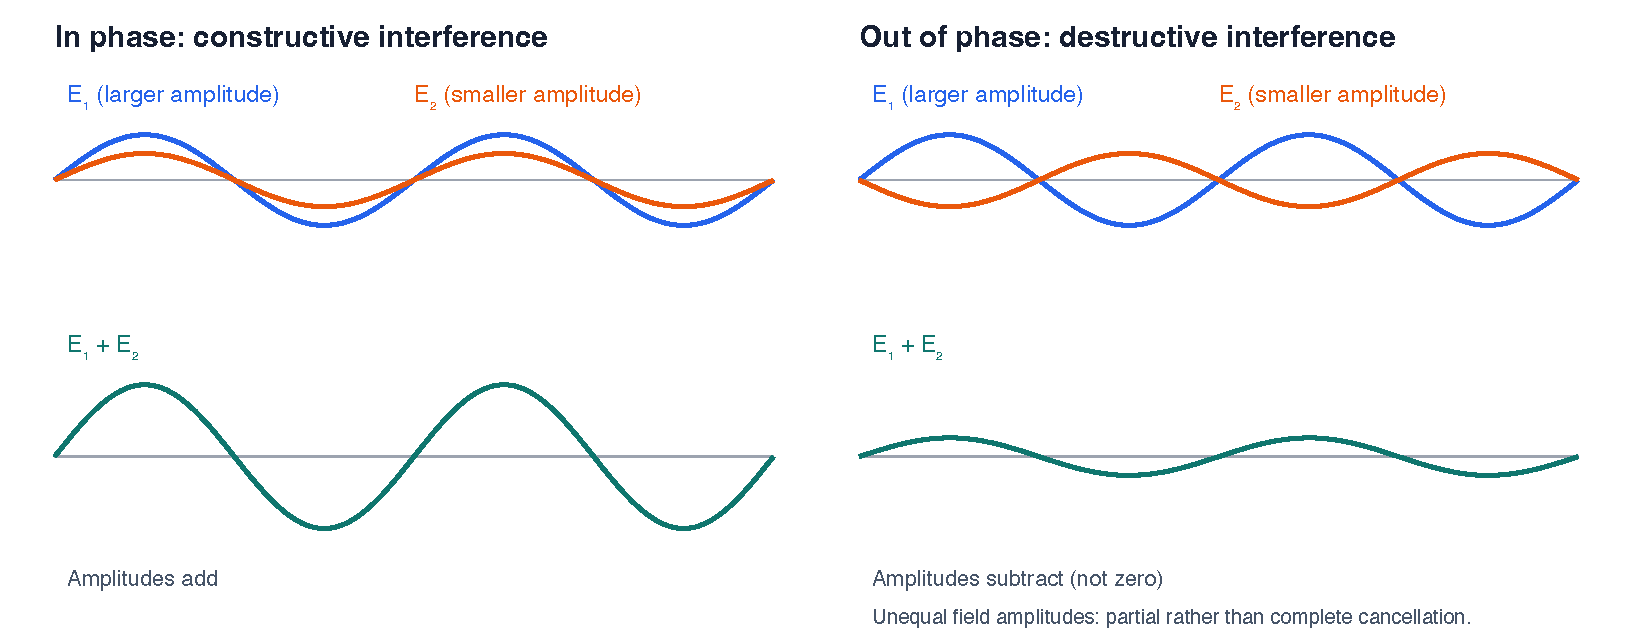
\includegraphics[width=0.90\linewidth]{figures/00_superposition.pdf}\vspace{-6pt}\end{center}
\begin{enumerate}
\item In the first example, why is the amplitude of $E_1+E_2$ larger than either individual field? What does this tell you about the relative phases of $E_1$ and $E_2$?
\answerspace{0.16in}
\item In the second example, why is the amplitude of $E_1+E_2$ smaller? What would change if the amplitudes of $E_1$ and $E_2$ were equal?
\answerspace{0.16in}
\end{enumerate}
\textbf{Optional resources:} \href{https://phet.colorado.edu/en/simulations/wave-interference}{PhET: Wave Interference} and \href{https://openstax.org/books/university-physics-volume-1/pages/16-5-interference-of-waves}{OpenStax: Interference of Waves}.
\newpage
\section*{Part B. How does interference make fringes?}
\begin{enumerate}[resume]
\item Two coherent waves arrive at the same point. Let $\Delta$ be their optical path difference and $\lambda$ the wavelength.

\textbf{(a)} What is the smallest nonnegative phase difference for constructive interference? For destructive interference?

\textbf{(b)} What path differences $\Delta$ produce constructive interference? What path differences produce destructive interference? Express your answers using $\lambda$.

\answerspace{0.12in}
\item The diagram shows two overlapping plane waves. Solid lines are \emph{crests}; dashed lines are \emph{troughs}. Adjacent crests of one wave are one wavelength apart.

\textbf{(a)} Identify the points where a crest from wave 1 meets a crest from wave 2. Mark several of these points on the diagram. What kind of interference occurs at these points?

\textbf{(b)} Identify the points where a trough from wave 1 meets a trough from wave 2. Mark several of these points on the diagram. What kind of interference occurs at these points?

\textbf{(c)} The vertical line at the right represents a screen. Mark the three locations on the screen where you predict bright fringes. Explain how you identified them from the wavefronts. Label the separation between neighboring bright fringes $d_0$.
\fig{0.84}{01_wavefronts}
\answerspace{0.02in}
\end{enumerate}

\newpage
\section*{Part C. Derive fringe spacing without a lens}
\begin{enumerate}[resume]
\item \textbf{Interference at one observation point.} The blue and orange lines represent crests of two overlapping plane waves. The screen has been positioned so that one blue crest and one orange crest intersect at $P$. The darker crests are reference crests of equal initial phase. The dashed segments $s_1$ and $s_2$ run from these reference crests to the \emph{same} observation point $P$, perpendicular to the respective wavefronts.
\fig{0.96}{02_geometry}
\textbf{(a)} What is the phase difference between the two waves at $P$? What kind of interference occurs there?

\textbf{(b)} Compare $s_1$ and $s_2$ using the symmetry of the diagram. What is the path difference $s_2-s_1$ at $P$? Explain why this agrees with your answer to (a).
\answerspace{0.32in}
\newpage
\noindent\textbf{Our strategy: comparing two bright fringes.}

At point $P$, the two waves interfere constructively. We want to understand how the
\emph{relative} distance traveled by the waves changes when we move down the screen
to the next bright fringe, $Q$.

\begin{enumerate}[label=\arabic*.,leftmargin=1.5em,itemsep=1pt,topsep=2pt]
\item For \textbf{wave 1}, compare the propagation distances to $P$ and $Q$:
$s_1'-s_1$.
\item For \textbf{wave 2}, make the same comparison: $s_2'-s_2$.
\item Subtract these two changes to find the change in \emph{relative} path difference:
\end{enumerate}
\vspace{-0.5em}
\[
\Delta s=(s_2'-s_2)-(s_1'-s_1).
\]
Because $P$ and $Q$ are adjacent bright fringes, the magnitude of this change is
one wavelength: $|\Delta s|=\lambda$. \textbf{Your task below} is to use geometry
to express these changes in terms of $d_0$ and $\theta$.

\medskip
\item \textbf{From one point to the next bright fringe.} In both diagrams, $P$ and $Q$ lie on the same screen, with $Q$ one bright-fringe spacing $d_0$ below $P$. Only crests are shown in these construction diagrams. The labels $s_1,s_1'$ refer to propagation distances for wave 1 at $P,Q$, and $s_2,s_2'$ to those for wave 2.

\textbf{(a) Wave 1 (example).} The dashed blue segments show the propagation distances $s_1$ and $s_1'$ to $P$ and $Q$. Both start on the same highlighted reference crest (but at different points) and run perpendicular to it. The right-triangle construction is a geometric aid. Which side gives the difference $s_1'-s_1$? Label that side, then use $\theta/2$ to express the difference in terms of $d_0$.
\begin{center}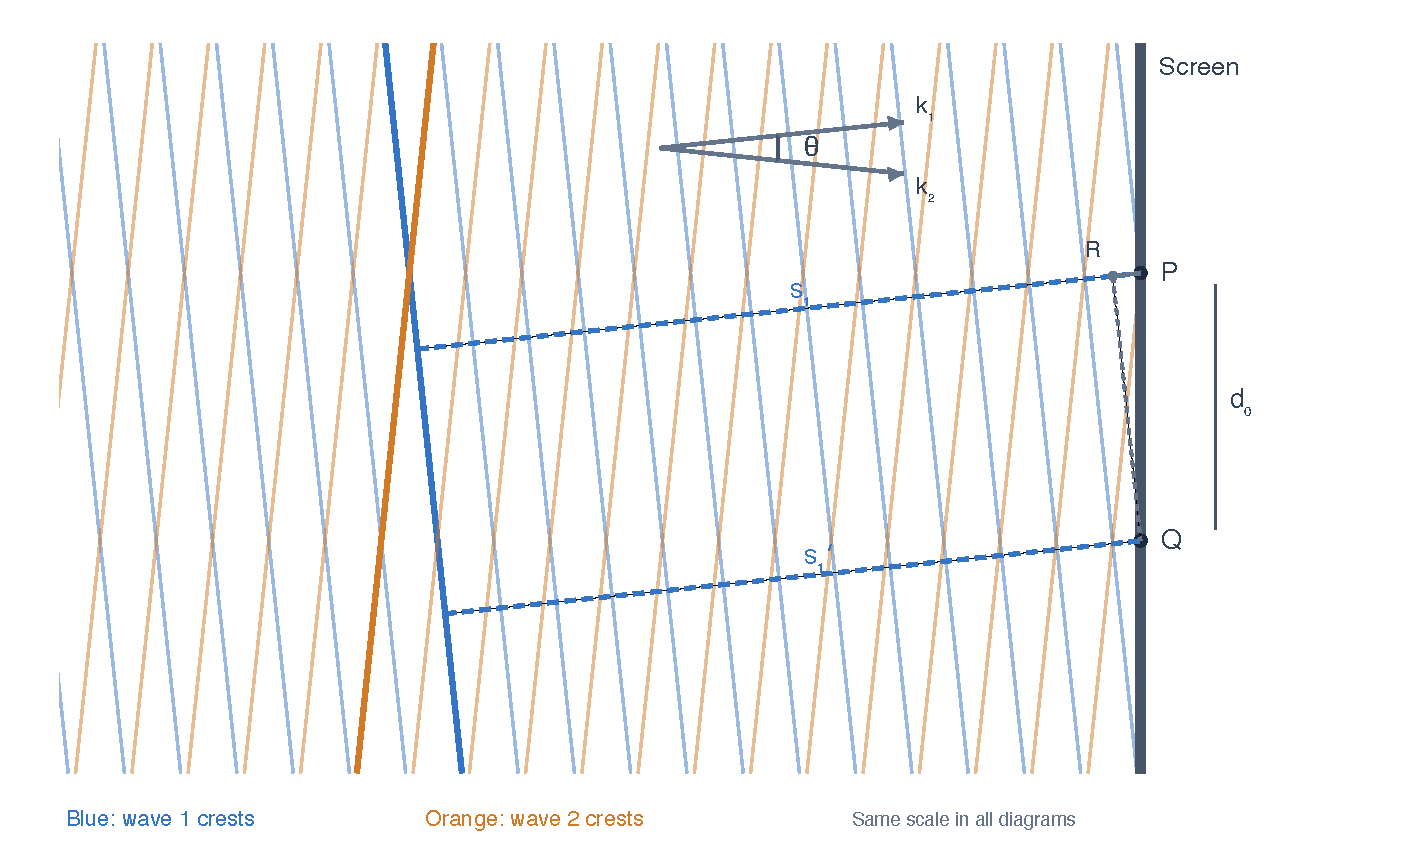
\includegraphics[width=0.96\linewidth]{figures/04_wave1.pdf}\end{center}
\textbf{(b) Wave 2 (your turn).} On the second diagram, draw the corresponding triangle for wave 2. The dashed orange segments show $s_2$ and $s_2'$. Draw the corresponding right triangle and mark the change $s_2'-s_2$ and determine its magnitude and sign relative to wave 1.
\begin{center}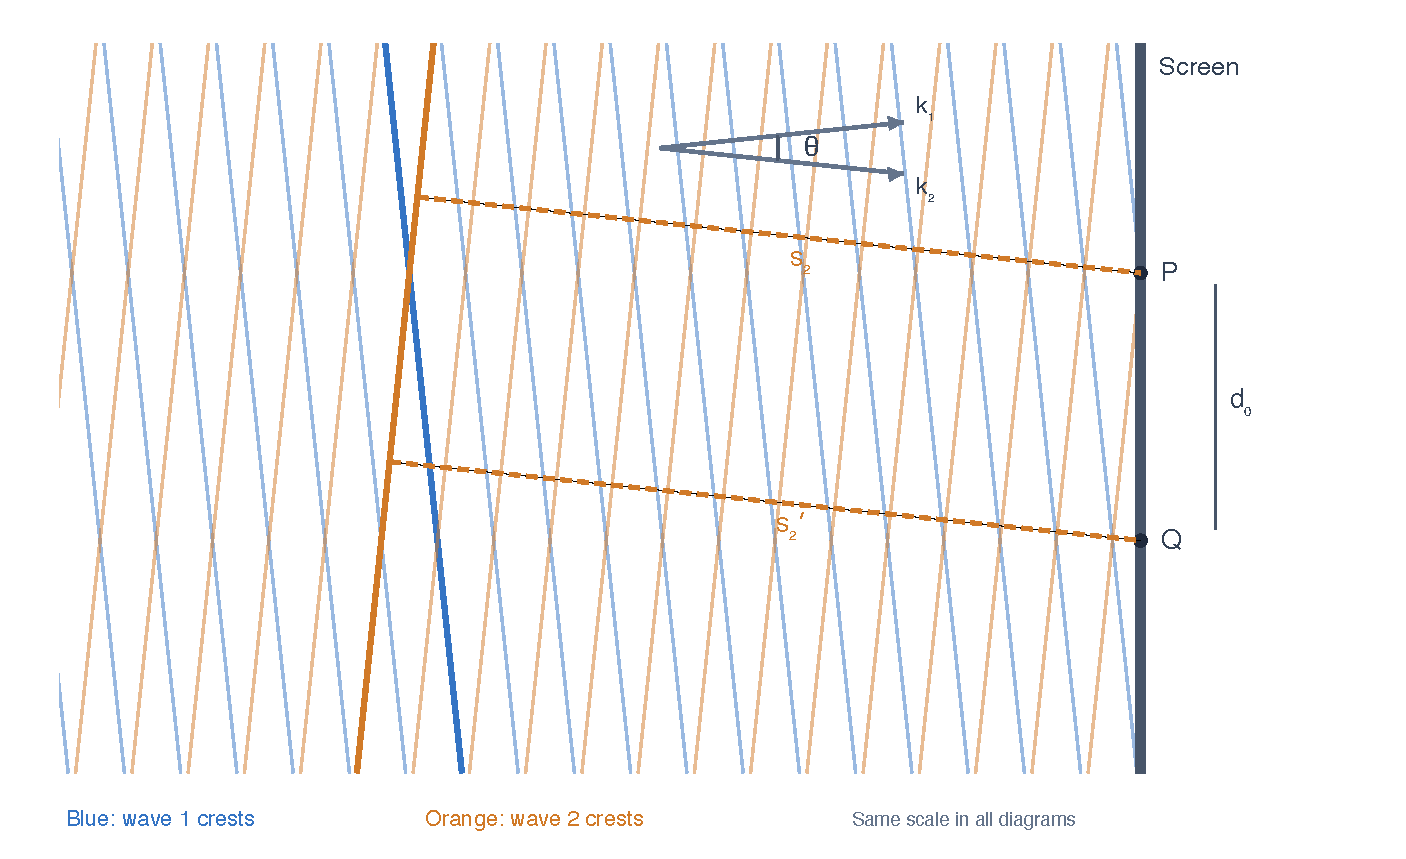
\includegraphics[width=0.96\linewidth]{figures/04_wave2_student.pdf}\end{center}
\textbf{(c)} Combine the two changes to find the change in \emph{relative} path difference between $P$ and $Q$. What must its magnitude equal for adjacent bright fringes? Use your triangles to derive the target result $d_0=\lambda/[2\sin(\theta/2)]$.
\answerspace{0.1in}
\item Let $d_0$ be the fringe spacing \emph{without} the lens. Summarize the geometric derivation from Question 5 and show the small-angle limit of
\[\boxed{d_0=\frac{\lambda}{2\sin(\theta/2)}\approx\frac{\lambda}{\theta}}\quad\text{for }\theta\text{ in radians and }\theta\ll1.\]
Write the algebra and identify where the small-angle approximation enters.
\answerspace{0.64in}
\item Does this ideal plane-wave expression contain the screen distance? Explain in words why moving the screen does not enlarge these fringes.
\answerspace{0.43in}
\end{enumerate}

\newpage
\section*{Part D. How can a lens enlarge the pattern?}
We now place a \emph{thin converging lens} after the second beam splitter. Let $D$ be the distance from the second beam splitter to the screen, $a$ the distance from the second beam splitter to the lens, and $L$ the distance from the lens to the screen. Therefore, $L=D-a$. We will use a geometrical-optics model of how a transverse coordinate is mapped from the lens plane to the screen. Avoid the focal plane ($L=f$), where this simple fringe-magnification model breaks down.
\begin{enumerate}[resume]
\item Two rays arrive at the lens parallel to the optical axis, at heights $y_1$ and $y_2$. On the diagram, continue the rays after the lens. Recall: a ray entering parallel to the axis passes through the back focal point, a distance $f$ beyond the lens. The back focal point $F$ is marked on the optical axis. Use it to trace the two refracted rays.
\fig{0.94}{03_lens_rays}
\noindent\textit{Figure:} Converging lens with focal length $f=75\,\mathrm{mm}$ and back focal point $F$. The drawing is not to scale: in the experiment, the screen is typically several meters beyond the lens.\par
\textbf{Ray-tracing help (click to open):} \href{https://phet.colorado.edu/en/simulations/geometric-optics-basics}{PhET: Geometric Optics: Basics} or \href{https://openstax.org/books/university-physics-volume-3/pages/2-4-thin-lenses}{OpenStax: Thin Lenses}, especially the two principal-ray rules.
\item Take a ray that hits the lens at height $y$. Using similar triangles, show that its height at a screen distance $L$ beyond the lens is
\[y_{\rm screen}=y\left(1-\frac{L}{f}\right).\]
Hint: the ray's slope immediately after the lens is approximately $-y/f$. Show your work.
\answerspace{0.62in}
\item Apply the same mapping to two nearby transverse positions separated by $d_0$. Show that the \emph{magnitude} of their separation on the screen is
\[\boxed{d_{\rm screen}=M d_0,\qquad M=\left|1-\frac{L}{f}\right|.}\]
Why do we need the absolute value? What happens when $L>f$?
\answerspace{0.54in}
\item Substitute $L=D-a$, then combine this result with Part C. Solve for the incoming beam angle $\theta$ in terms of $\lambda$, $d_{\rm screen}$, $D$, $a$, and $f$. Circle your final result.
\answerspace{0.82in}
\end{enumerate}

\section*{Part E. Your measurement}
\begin{enumerate}[resume]
\item Record the values below, convert all lengths to meters, and calculate $M$ and $\theta$. Use radians for the angle, then convert to degrees.
\[\begin{array}{rcl@{\qquad}rcl}
\lambda&=&\underline{\hspace{1.2in}}&f&=&\underline{\hspace{1.2in}}\\[12pt]
D&=&\underline{\hspace{1.2in}}&a&=&\underline{\hspace{1.2in}}\\[12pt]
d_{\rm screen}&=&\underline{\hspace{1.2in}}&M&=&\underline{\hspace{1.2in}}
\end{array}\]
\answerspace{0.6in}
\item \textbf{Approximation and uncertainty.} For $D\gg f,a$, use
\[\theta\approx\frac{\lambda D}{f\,d_{\rm screen}}.\]
\textbf{(a)} The general propagation-of-uncertainty formula for independent measurements is
\[\sigma_q=\sqrt{\sum_i\left(\frac{\partial q}{\partial z_i}\sigma_{z_i}\right)^2},\]
where $q=q(z_1,z_2,\ldots)$ and $\sigma_{z_i}$ is the standard uncertainty in $z_i$.
Apply this formula to $\theta$ and write an expression for the \emph{fractional uncertainty} $\sigma_\theta/\theta$ in terms of the fractional uncertainties in $\lambda$, $D$, $f$, and $d_{\rm screen}$. Show the partial derivatives or your intermediate steps; do not skip straight to the simplified answer.
\smallskip
\noindent\textbf{Worked examples (optional):} \href{https://physicslabs.colorado.edu/courses/python/data-analysis/error-propagation}{CU Boulder: Error Propagation with Python} (derivatives and independent uncertainties); \href{https://www.physics.wisc.edu/instructional/LabManuals/Archive/UWPhysics202Fall22LabManual.pdf}{Wisconsin Physics 202 Lab Manual} (worked examples of fractional uncertainties).
\par\smallskip
\textbf{(b)} If the wavelength and focal length are treated as exact compared with the measured distances, explain which terms can be neglected. Simplify your expression to include only $\sigma_D/D$ and $\sigma_d/d_{\rm screen}$.
\textbf{(c)} Which measured quantity contributes more to your uncertainty in $\theta$? Justify your answer using fractional uncertainties, not absolute uncertainties.
\smallskip
\answerspace{1.45in}
\item \textbf{Concept check: moving the screen.} Suppose you move the screen farther away from the second beam splitter, without changing the lens or the alignment of the interferometer.

\textbf{(a)} Would the distance between adjacent bright fringes increase, decrease, or stay the same?

\textbf{(b)} Explain your prediction using the fringe-spacing equation you derived. Assume the screen remains well beyond the focal plane of the lens.
\answerspace{0.62in}
\end{enumerate}
\vfill
\small\textit{Model limitation:} The lens derivation uses paraxial rays and the geometrical mapping of a locally periodic pattern. It assumes sufficient overlap and coherence of the two beams at the screen. Near the focal plane, or for strongly curved/unequal input wavefronts, a fuller wave-optics treatment is needed.
\end{document}
